% kapitel4.tex
\chapter{Wagner Struktur}
\label{cha:wagnerstruktur}

In diesem Kapitel soll Theorem \ref{eq:Theorem36} genauer betrachtet werden.
Es ist, wie erwähnt, auf Wagner zurückzuführen:
\begin{theorem}\label{eq:TheoremWagner}
  Ein Graph enthält genau dann keinen \kf-Minor, wenn er ein Teilgraph eines Graphen ist, der aus planaren Graphen und Kopien von $W$ erzeugt werden kann, welche an Cliquen zusammengeführt wurden.\cite{Wag37}
\end{theorem}
Als Beispiel ist dazu in Abbildung \ref{fig:WagnerStruktur1} ein Graph $G$ zu sehen, der nicht planar ist, aber keinen \kf-Minor enthält und nach dem Theorem aus $G'$ aus Abbildung \ref{fig:WagnerStruktur2} ein zu $G$ isomorpher Teilgraph erzeugt werden kann.
$G'$ enthält nur planare Zusammenhangskomponenten \bzw eine, die isomorph zu $W$ ist.
Einige Cliquen sind hier mit je einer Farbe hervorgehoben, sodass durch das Zusammenfügen gleichfarbiger Knoten ein Graph $G''$ erzeugt werden kann, der $G$ als Teilgraph enthält.
Zusätzlich bilden in $G''$ die roten Knoten eine Clique, in $G$ sind sie nicht adjazent.
Um einen isomorphen Graph zu erhalten, muss $G'$ durch Cliquen-Summen erzeugt werden, da bei der Operation Kanten zwischen Cliquenknoten im Anschluss entfernt werden dürfen.
Somit kann Theorem \ref{eq:TheoremWagner} so umforumliert werden, dass jeder Graph ohne \kf-Minor durch Cliquen-Summen von planaren Graphen und Kopien von $W$ erzeugt werden kann.
Problematisch ist allerdings, dass eine Cliquen-Summe nicht festlegt, ob und welche Kanten innerhalb der Clique gelöscht werden.
Das Theorem kann aber genutzt werden, um einen Graph in seine planaren Komponenten und Kopien von $W$ aufzuteilen, sollte er keinen \kf-Minor enthalten.

\begin{figure}[H]
  \centering
  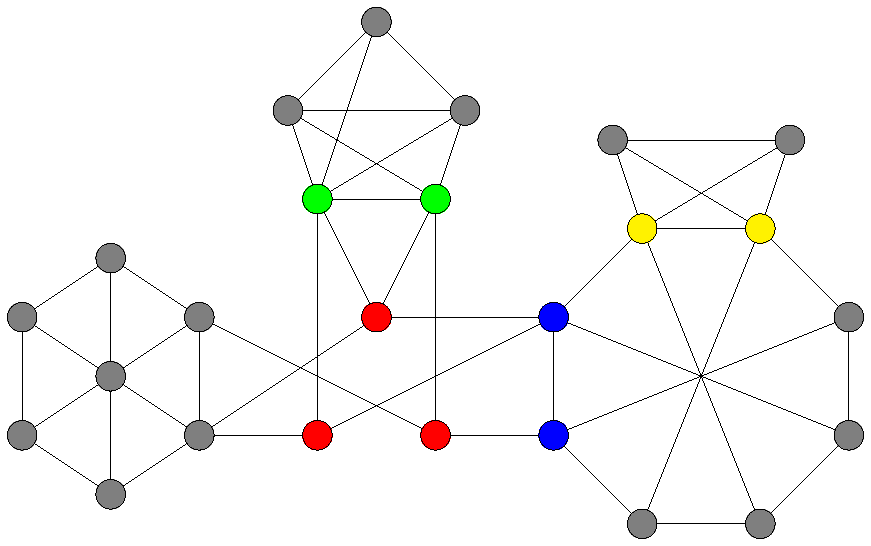
\includegraphics[width=\textwidth,height=\textheight,keepaspectratio]{bilder/WagnerTheorem1.pdf}
  \caption{Ein nicht-planarer Graph $G$, der keinen \kf-Minor enthält.}
  \label{fig:WagnerStruktur1}
\end{figure}

\begin{figure}[H]
  \centering
  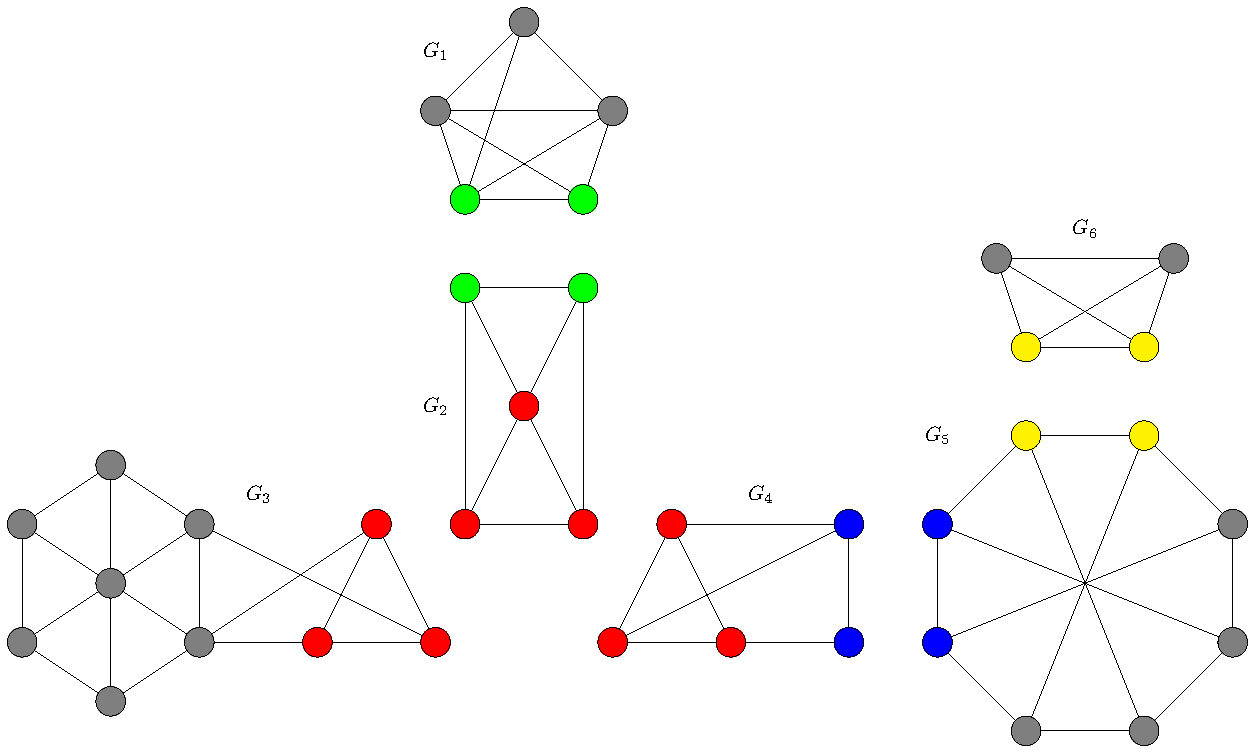
\includegraphics[width=\textwidth,height=\textheight,keepaspectratio]{bilder/WagnerTheorem2.pdf}
  \caption{Ein nicht zusammenhängender Graph $G'$, dessen Zusammenhangskomponenten planar oder isomorph zu $W$ sind.}
  \label{fig:WagnerStruktur2}
\end{figure}

Um die im Theorem beschriebene Struktur - im Folgenden als \textit{Wagner-Struktur} bezeichnet - aufzubauen, werden einige Baumstrukturen betrachtet, die den $2$- und $3$-Zusammenhang in Graphen herstellen sowie die $(3, 3)$-Separatoren behandeln.
Zunächst werden Block-Cut Trees und $1$-Block-Trees vorgestellt, die im Zusammenhang mit den durch $1$-Separatoren erzeugen augmentierten Komponenten von Kezdy und McGuinness stehen.
Anschließend werden SPQR-Bäume und $2$-Block-Trees für augmentierte Komponenten mit $2$-Separatoren und $(3, 3)$-Block-Trees für solche mit $(3, 3)$-Separatoren erklärt.
Letztlich wird genauer auf den Zusammenhang zwischen dem Algorithmus von Kezdy und McGuinness, den unterschiedlichen Baumstrukturen und der Wagner-Struktur eingegangen.
Es sei außerdem erwähnt, dass sowohl Block-Cut Trees als auch SPQR-Bäume bereits in \OGDF implementiert sind - demgegenüber werden $1$-, $2$- und $(3, 3)$-Block-Trees hier als theoretische Konstrukte benutzt, um eine Wagner-Struktur besser abbilden zu können.
Das Ziel der Wagner-Struktur soll sein, als Zertifikat für Graphen zu dienen, wenn sie \kf-Minor frei sind.
Andernfalls kann der gefundene \kf-Minor als Zertifikat benutzt werden.

% 1-Block-Tree
\begin{wrapfigure}{r}{6cm}
  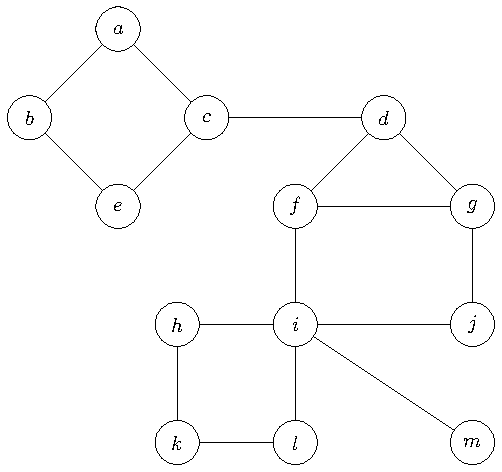
\includegraphics[width=6cm]{bilder/1-Block-Tree1.pdf}
  \caption{Ein nicht $2$-zusammenhängender Graph $G_1$.}
  \label{fig:1-Block-Tree1}
\end{wrapfigure}
\textbf{Block-Cut-Tree}: Als \textit{Block} eines Graphen $G$ wird jeder seiner maximalen Teilgraphen bezeichnet, der keinen $1$-Separator enthält - als $2$-zusammenhängend ist.
Je zwei Blöcke haben maximal einen gemeinsamen Knoten, der einen $1$-Separator in $G$ bildet.\cite{BoM08}
Ein Block-Cut Tree ist ein Baum, der für jeden Block von $G$ einen Knoten besitzt und für jeden Separator eine Kante.
Als Beispiel wird in Abbildung \ref{fig:1-Block-Tree1} ein Graph mit dazugehörigem Block-Cut Tree in Abbildung \ref{fig:1-Block-Tree2} gezeigt.
Die Knoten des Block-Cut Tree sind als durchgezogene Linien angegeben, in jedem dieser Knoten findet sich ein $2$-zusammenhängender Teilgraph aus $G_1$. %TODO: Laufzeit
\begin{figure}[H]
  \centering
  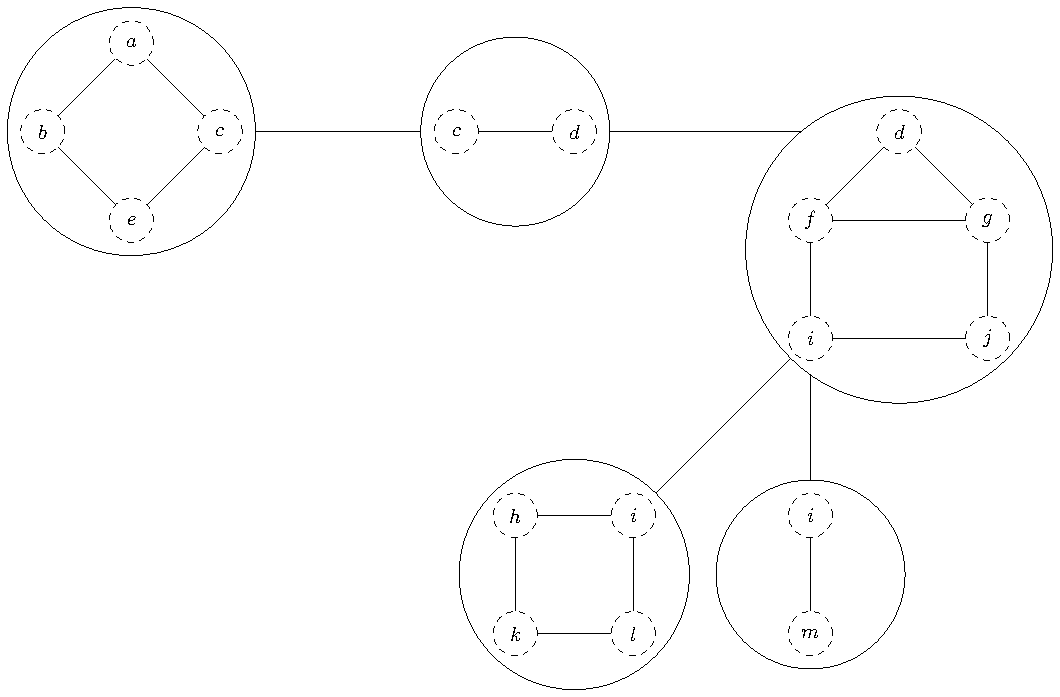
\includegraphics[width=\textwidth,height=\textheight,keepaspectratio]{bilder/1-Block-Tree2.pdf}
  \caption{Der Block-Cut Tree zu $G$ aus Abbildung \ref{fig:1-Block-Tree1}.}
  \label{fig:1-Block-Tree2}
\end{figure}

In \cite{Li11} stellt Li eine Erweiterung zum Block-Cut Tree vor, die als \textit{$1$-Block-Tree} bezeichnet wird, da neben den Blöcken auch $1$-Separatoren enthalten sind.

\textbf{$1$-Block-Tree}: Seien für einen Graph $G$ die Knoten seines Block-Cut Trees $T_C$ als Blockknoten bezeichnet.
Dann enthält der $1$-Block-Tree $T_1$ von $G$ statt jeder Kante, die zwei Blockknoten $u$ und $v$ in $T_C$ verbindet, die Kanten $(u, c)$ und $(c, v)$, wobei $c$ als Cliquenknoten bezeichnet wird und den $1$-Separator beinhaltet, den die zu $u$ und $v$ zugehörigen Teilgraphen in $G$ als gemeinsamen Knoten besitzen.
Ein Beispiel findet sich in Abbildung \ref{fig:1-Block-Tree3}.
Es kann beobachtet werden, dass die in Blockknoten enthaltenen Teilgraphen identisch zu den augmentierten Komponenten sind, die im Algorithmus von Kezdy und McGuinness in Schritt \ref{item:algorithmus11} durch $1$-Separatoren gebildet werden.
\begin{figure}[H]
  \centering
  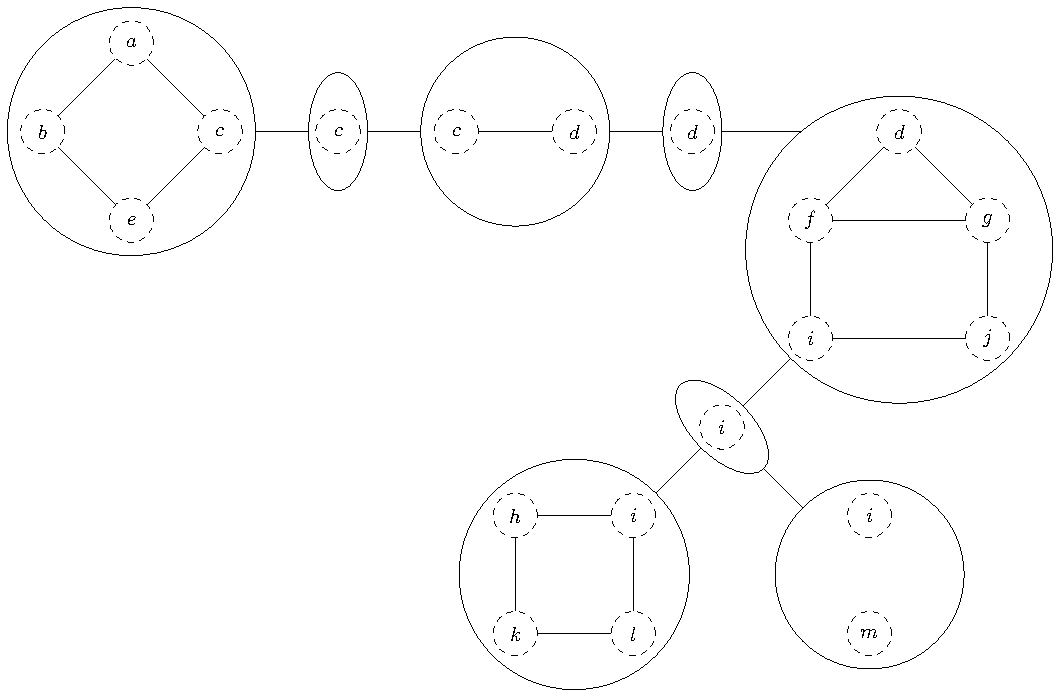
\includegraphics[width=\textwidth,height=\textheight,keepaspectratio]{bilder/1-Block-Tree3.pdf}
  \caption{Der $1$-Block-Tree zu $G$ aus Abbildung \ref{fig:1-Block-Tree2}.
           Die Cliquenknoten sind ovalförmig dargestellt.}
  \label{fig:1-Block-Tree3}
\end{figure}


% 2-Block-Tree
Nachdem durch Block-Cut Trees \bzw $1$-Block-Trees der $2$-Zusammenhang in allen Blockknoten hergestellt wurde, können die darin enthaltenen Teilgraphen jeweils als Eingabe für einen SPQR-Baum genutzt werden, um $3$-zusammenhängende Komponenten zu erzeugen.
Die folgende Definition dazu ist \cite{GuM00} entnommen.

\begin{figure}[H]
  \centering
  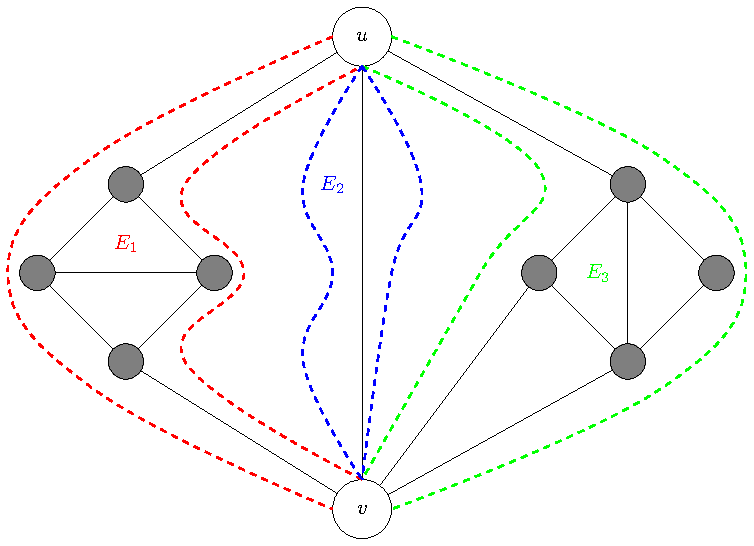
\includegraphics[width=\textwidth,height=\textheight,keepaspectratio]{bilder/Split-Kantenmengen.pdf}
  \caption{Unterteilung der Kanten in drei Mengen $E_1$, $E_2$ und $E_3$ anhand des Knotenpaares $\{u, v\}$.}
  \label{fig:Split-Kantenmengen}
\end{figure}

\textbf{SPQR-Baum}: Sei $G = (V, E)$ ein $2$-zusammenhängender Graph, betrachtet werden alle Knotenpaare $\{u, v\}$ in $G$, die entweder benachbart sind oder einen $2$-Separtoren bilden.
Dieses Knotenpaar teilt die Kanten in die Mengen $E_1, ..., E_k$, sodass eine Menge $E_i$ alle Pfade enthält, die $u$ oder $v$ höchstens als Endpunkte haben.
In \Abb \ref{fig:Split-Kantenmengen} ist ein $2$-zusammenhängender Graph skizziert, in dem $\{u, v\}$ eingezeichnet ist, sowie farblich hervorgehoben die dadurch entstehende Unterteilung in Kantenmengen.
Jeder Knoten des SPQR-Baums von $G$ wird durch diese Kantenmengen festgelegt, und je nach Eigenschaft entweder mit \textit{S}, \textit{P}, \textit{Q} oder \textit{R} markiert:
\begin{itemize}
  \item \textbf{Q}: Tritt der Randfall auf, dass $G$ nur eine einzige Kante $(u, v)$ besitzt,dann enthält der SPQR-Baum einen einzelnen Q-Knoten, der auf $G$ verweist.
  \item \textbf{P}: Entstehen durch das Knotenpaar die Kantenmengen $E_1, ..., E_k$ mit $k \geq 3$, dann wird ein P-Knoten hinzugefügt, der das Knotenpaar enthält sowie $k$ viele parallele Kanten zwischen diesem.
  \item \textbf{S}: Andernfalls teilen $u$ und $v$ die Kanten in zwei Mengen, sodass es zwei unterschiedliche Pfade gibt, die das Knotenpaar verbinden.
                    Der hinzugefügte S-Knoten enthält das Knotenpaar sowie diese beiden Pfade.
  \item \textbf{R}: Tritt keiner der obigen Fälle ein, dann wird in je einem R-Knoten der maximale $3$-zusammenhängende Teilgraph gespeichert, der $\{u, v\}$ enthält.
                    Zusätzlich wird die Kante $(u, v)$ hinzugefügt, falls sie noch nicht vorhanden ist.
\end{itemize}

\begin{figure}[H]
  \centering
  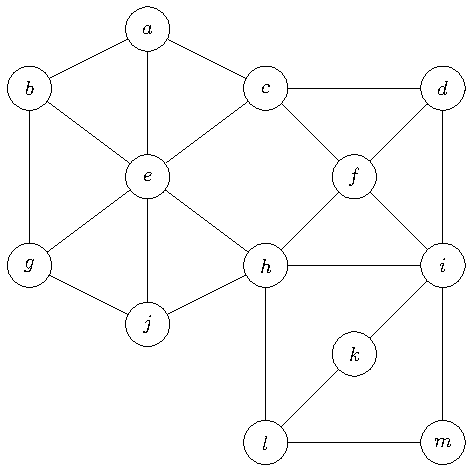
\includegraphics[width=8cm]{bilder/2-Block-Tree1.pdf}
  \caption{Ein $2$-zusammenhängender Graph $G_2$.}
  \label{fig:2-Block-Tree1}
\end{figure}

\begin{figure}[H]
  \centering
  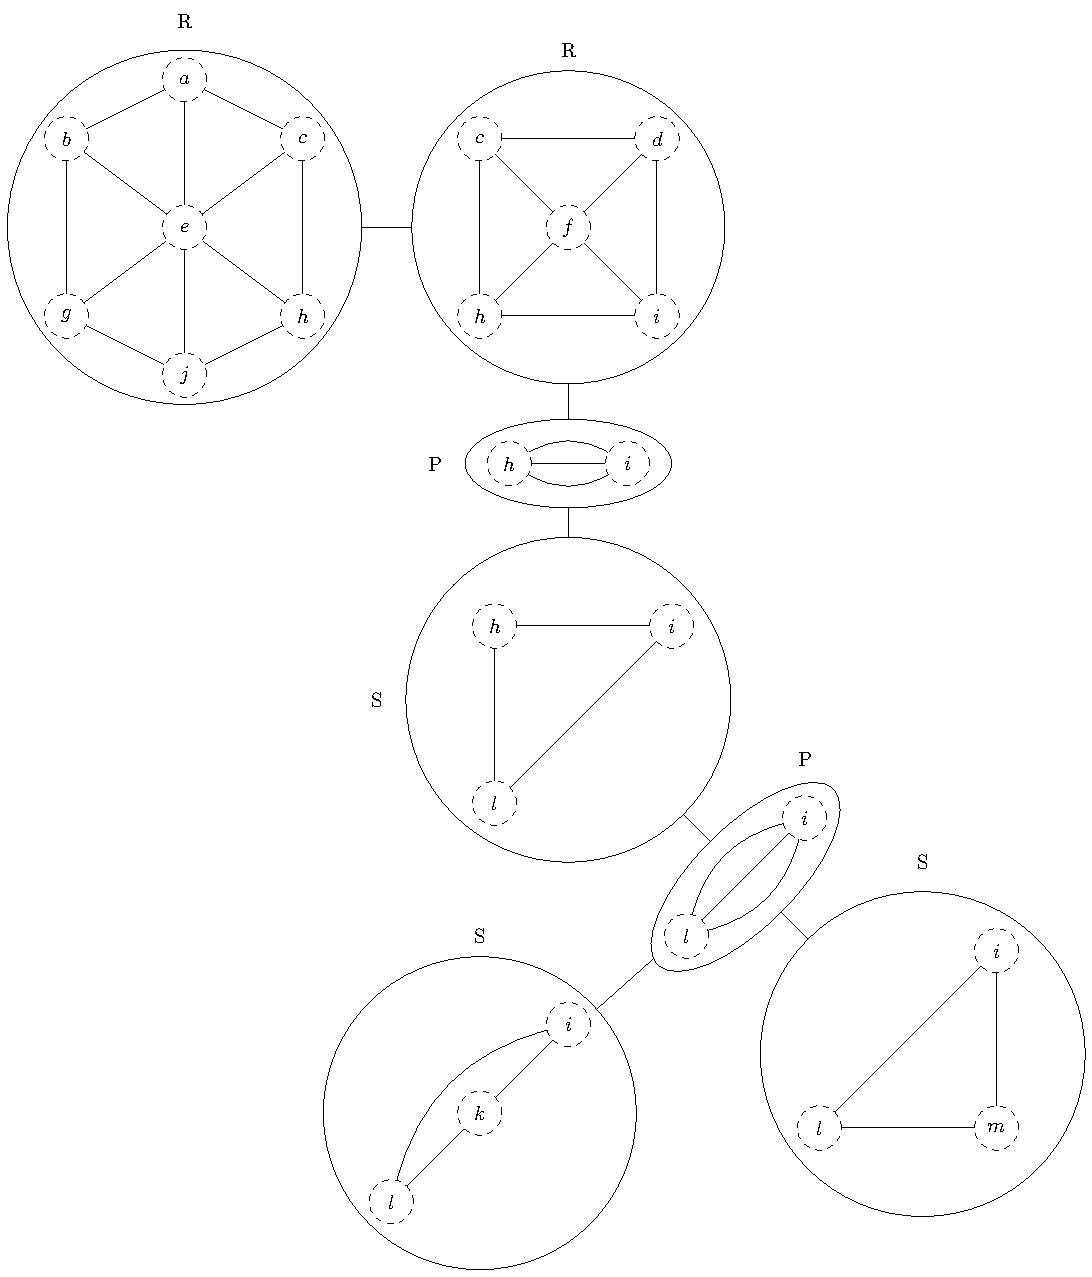
\includegraphics[width=\textwidth,height=\textheight,keepaspectratio]{bilder/SPQR-Tree.pdf}
  \caption{SPQR Baum zum Graph $G_2$ aus \Abb \ref{fig:2-Block-Tree1}.}
  \label{fig:SPQR-Tree}
\end{figure}

Zu dem Graph in \Abb \ref{fig:2-Block-Tree1} ist in \Abb \ref{fig:SPQR-Tree} der zugehörige SPQR Baum skizziert.
Erkennbar sind zwei R-Knoten, die $3$-zusammenhängende Minoren von $G_2$ sind.
Außerdem sind drei Kreisgraphen enthalten (S-Knoten) und zwei P-Knoten mit parallelen Kanten. % TODO: P Knoten (c, h)

In Bezug auf den Algorithmus von Kezdy und McGuinness sind vor allem die R-Knoten interessant, da sie die $3$-zusammenhängenden Komponenten eines Graphen enthalten.
Vielmehr bilden sie sogar genau die augmentierten Komponenten, die im Algorithmus in Schritt \ref{item:algorithmus12} erzeugt werden mit Außnahme von Kreisen der Größe drei.
Jeder R-Knoten besteht aus einem $3$-zusammenhängenden Teilgraph, wobei darin enthaltene Knotenpaare, die $2$-Separatoren im ursprünglichen Graph gebildet haben, in den Teilgraphen immer adjazent sind.
Die übrigen Knoten des SPQR-Baumes werden nicht benötigt:
Q- und P-Knoten sind immer planar und müssen nicht weiter beachtet werden.
S-Knoten können, wie etwa in \Abb \ref{fig:SPQR-Tree}, ebenfalls gültige augmentierte Komponenten enthalten.
Allerdings handelt es sich dabei ausschließlich um Kreise, welche ebenfalls immer planar sind.

In \cite{Li11} stellt Li analog zum $1$-Block-Tree den $2$-Block-Tree vor, der aus $3$-zusammenhängende Komponenten (Blockknoten) und $2$-Separatoren (Cliquenknoten) besteht.

\textbf{$2$-Block-Tree}: Sei $G = (V_G, E_G)$ ein $2$-zusammenhängender, \kf-Minor freier Graph und $T_2 = (V_T, E_T)$ der $2$-Block-Tree.
Bilden die Knoten $u, v \in V_G$ einen $(2, j)$-Separator in $G$ für $j \geq 2$, dann seien erneut $Z_1, ..., Z_j$ die Zusammenhangskomponenten von $G - \{u, v\}$.
Analog zum $1$-Block-Tree wird ein Cliquenknoten für den Separator angelegt, der alle Blockknoten bestehend aus $Z_i \cup \{u, v\}$ als Nachbarn besitzt.
Außerdem wird die Kante $(u, v)$ sowohl in den Block- als auch in dem Cliquenknoten hinzugefügt, falls sie nicht vorhanden ist.
Ist $G$ $3$-zusammenhängend, besitzt $T_2$ einen einzelnen Blockknoten, der $G$ vollständig enthält.
Ein $2$-Block-Tree zu $G_2$ aus \Abb \ref{fig:2-Block-Tree1} ist in \Abb \ref{fig:2-Block-Tree2} zu sehen.
Es ist zu beobachten, dass Knoten wie etwa $h$ oder $i$ Teil mehrerer Separatoren sein können und somit nicht nur in mehreren Graph-, sondern auch in mehreren Cliquenknoten enthalten sind.
Allerdings sind keine zwei Knoten im $2$-Block-Tree identisch.
\begin{figure}[H]
  \centering
  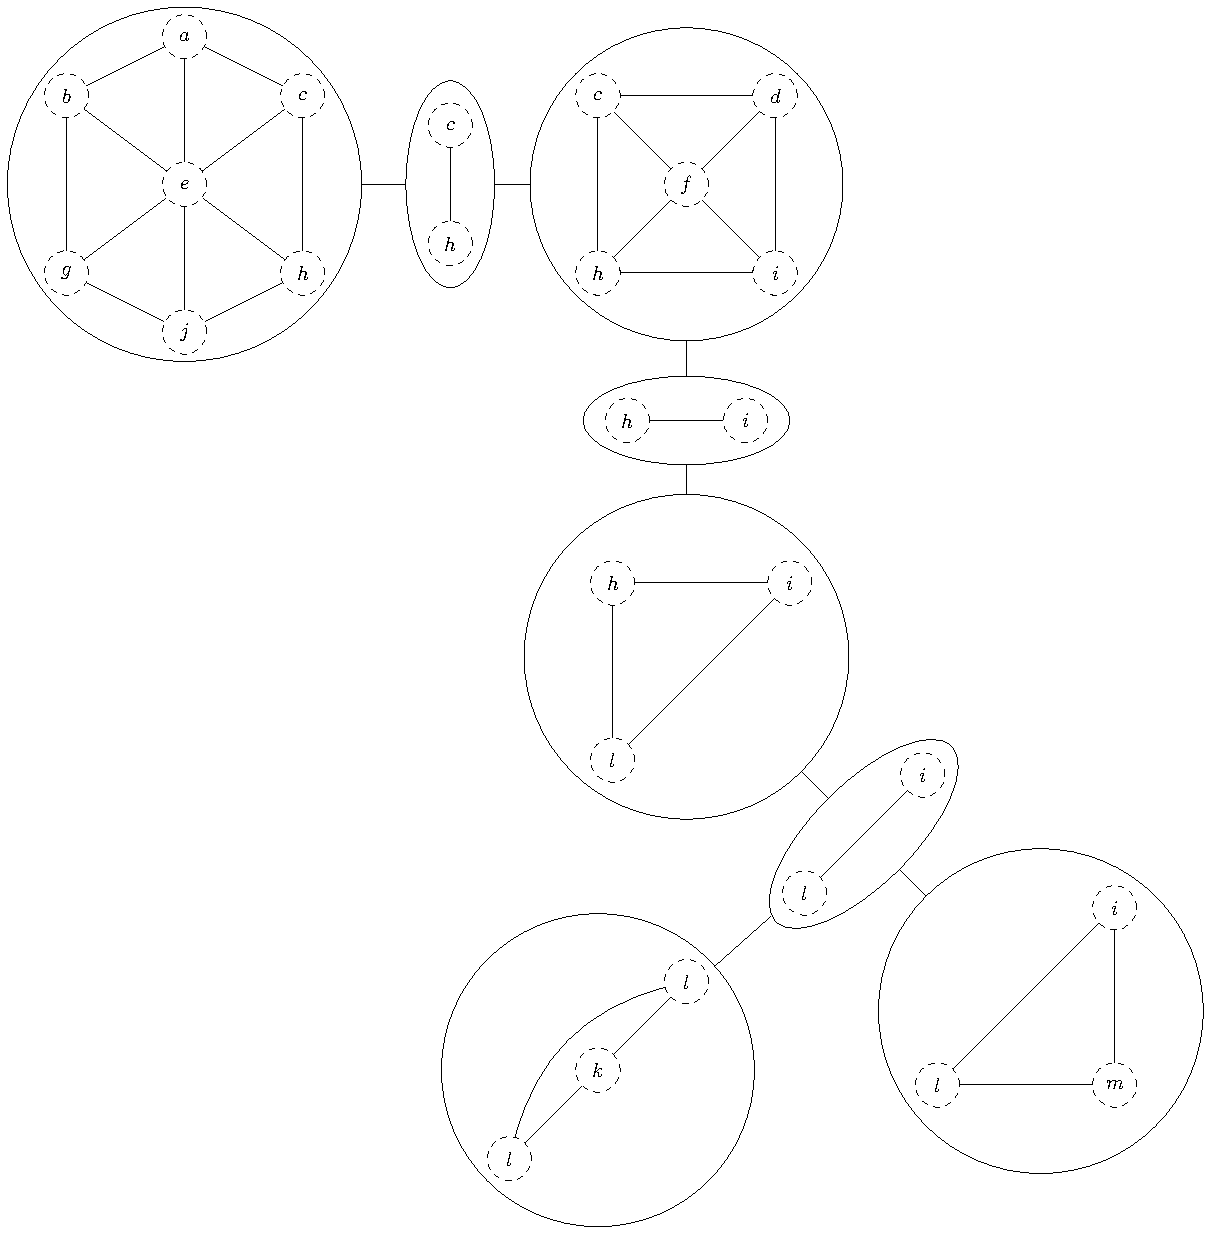
\includegraphics[width=\textwidth,height=\textheight,keepaspectratio]{bilder/2-Block-Tree2.pdf}
  \caption{$2$-Block-Tree zum Graph aus \Abb \ref{fig:2-Block-Tree1}.
           Die Cliquenknoten sind ovalförmig dargestellt und enthalten immer genau zwei Knoten, alle übrigen sind Blockknoten.}
  \label{fig:2-Block-Tree2}
\end{figure}


% (3, 3)-Block-Tree
\textbf{$(3, 3)$-Block-Tree}: Sei $G = (V_G, E_G)$ ein $3$-zusammenhängender, \kf-Minor freier Graph und $T_{(3, 3)} = (V_T, E_T)$ der $(3, 3)$-Block-Tree.
Enthält $G$ keinen $(3, j)$-Separator für $j \geq 3$, so besitzt $T_{(3, 3)}$ einen einzigen Blockknoten, der $G$ komplett enthält.
Sei andernfalls $C$ ein Graph, der die drei Knoten eines solchen $(3, j)$-Separators als Clique beinhaltet.
Dann werden Blockknoten in $T_{(3, 3)}$ für alle $Z_i \cup C$ mit $1 \leq i \leq j$ angelegt, wobei $Z_i$ die durch den Separator entstandenen Zusammenhangskomponenten sind.
Außerdem wird ein Cliquenknoten mit $C$ erzeugt, der im Baum Kanten zu allen zuvor erzeugten Blockknoten hat.
Ein Beispiel ist in Abbildung \ref{fig:33-Block-Tree} skizziert.
\begin{figure}[H]
  \centering
  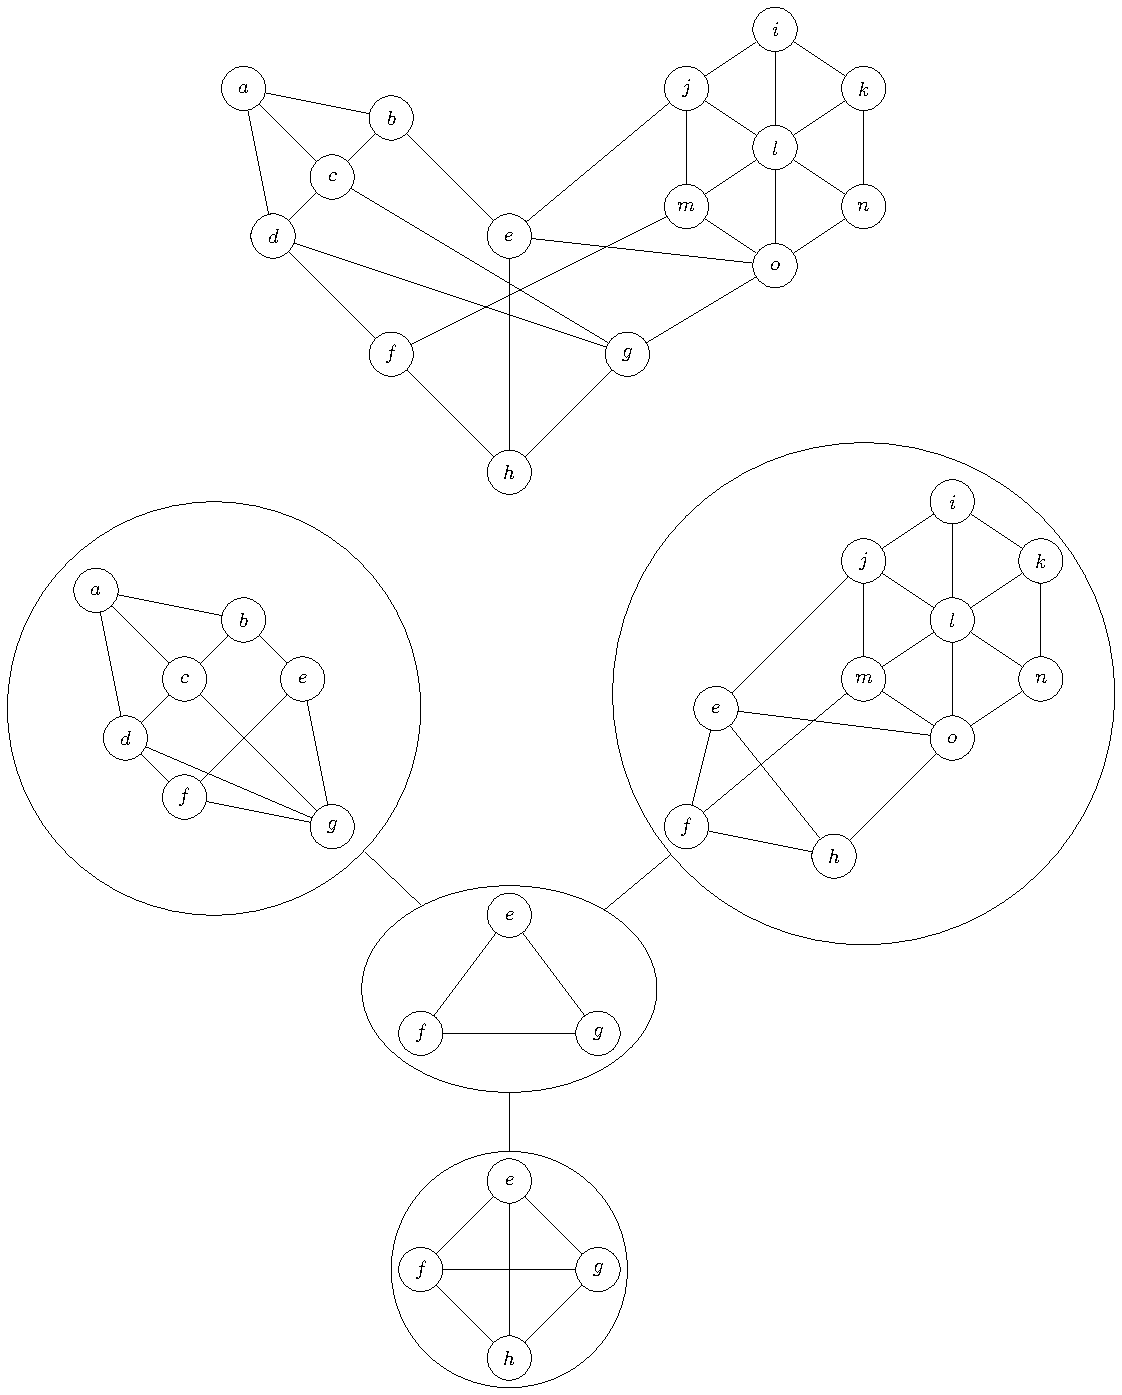
\includegraphics[width=\textwidth,height=\textheight,keepaspectratio]{bilder/33-Block-Tree.pdf}
  \caption{Ein $3$-zusammenhängender Graph mit dazugehörigem $(3, 3)$-Block-Tree.
           Der Separator wird durch $\{e, f, g\}$ gebildet.
           Es ist zu sehen, dass der Eingabegraph nicht planar ist, da ein \kdd-Minor enthalten ist.
           Die Blockknoten enthalten jedoch alle planare Minoren des ursprünglichen Graphs.}
  \label{fig:33-Block-Tree}
\end{figure}


Um nun aus einem schlichten nicht zusammenhängenden Graph $G$ ohne \kf-Minor eine Wagner-Struktur zu erzeugen, wird zunächst für jede Zusammenhangskomponente ein $1$-Block-Tree $T_1$ angelegt.
Jeder Blockknoten $t \in T_1$ beinhaltet einen $2$-zusammenhängenden Teilgraph $G'$ von $G$, welcher als Eingabe für einen $2$-Block-Tree $T_2$ dient.
Ist $G$ bereits $2$- \bzw $3$-zusammenhängend, kann der entsprechende Block-Tree übersprungen und $G$ direkt als Eingabe für den $2$- \bzw $(3, 3)$-Block-Tree verwendet werden.
Anschließend kann jeder $3$-zusammenhängende Teilgraph $G''$, der mit einem Blockknoten von $T_2$ assoziiert wird, als Eingabe für einen $(3, 3)$-Block-Tree verwendet werden.
Dadurch entsteht ein Baum, der zeigt, wie nach Theorem \ref{eq:TheoremWagner} der Graph $G$ aus planaren Graphen und Kopien von $W$ (Blockknoten) durch Cliquen-Summen (Cliquenknoten) erzeugt werden kann.
Zwar ist der Eingabegraph nicht immer eindeutig aus der Wagner-Struktur wiederherstellbar, allerdings ist die relevante Eigenschaft einer solchen Struktur vielmehr, dass sie nur für \kf-Minor freie Graphen existiert.
Scheitert der Aufbau einer Wagner-Struktur, ist der Graph nicht \kf-Minor frei.


\section{Algorithmus von Kezdy und McGuinness als Wagner-Struktur}
Im Folgenden wird die Wagner-Struktur von Reed und Li mit dem Algorithmus von Kezdy und McGuinness verglichen und dieser so modifiziert, dass er sie erzeugen kann.
Anschließend werden augmentierte Komponenten für $1$- und $2$-Separatoren durch Block-Cut Trees und SPQR-Bäume erzeugt sowie ein zertifizierender Algorithmus beschrieben.

\subsection{Block-Trees}
\textbf{Behauptung:} Wird der Graph in augmentierte Komponenten aufgeteilt, sind diese genau dann isomorph zu mindestens einem Blockknoten der verschiedenen Block-Trees, wenn alle Separatoren gleich gewählt wurden.
Im Algorithmus von Kezdy und McGuinness wird der Graph in augmentierte Komponenten aufgeteilt, wenn ein $(1, 2)$-, $(2, 2)$- oder $(3, 3)$-Separator gefunden wird.

Sei $C$ ein solcher $(i, j)$-Separator, der einen zusammenhängenden Graph $G$ in genau $j$ Zusammenhangskomponenten $Z_1, ..., Z_j$ aufteilt, wenn die $i$ Knoten von $C$ aus $G$ entfernt werden.

Angenommen, es gäbe eine augmentierte Komponenten $G_a$, zu der es im zugehörigen $(3, 3)$-Block-Tree keinen Blockknoten $t$ mit assoziiertem Graph $G_t$ gibt, sodass $G_a$ und $G_t$ isomorph sind.
Dann gibt es einen Separator $C_a$ in $G$, aus dem $G_a$ entstanden ist.
Da es kein $t$ mit einem zu $G_a$ isomorphen $G_t$ gibt, wurden keine Knoten im Block-Tree mit $C_a$ erzeugt, sodass es ebenfalls keinen Cliquenknoten mit $C_a$ gibt.
Dann wurde mindestens ein Separator $C_a'$ für den $1$-Block-Tree gewählt, wodurch die Knoten von $C_a$ so in Blockknoten enthalten sind, dass sie dort keinen Separator bilden, was der gleichen Wahl von Separatoren widerspricht.
Oder $C_a$ ist vollständig in einem Blockknoten enthalten und bildet dort einen Separator, was entweder dem $2$-Zusammenhang oder der Planarität \bzw Isomorphie zu $W$ des Blockknotens widerspricht.

Der Algorithmus von Kezdy und McGuinness erzeugt also zu Beginn alle Blockknoten eines $1$-Block-Trees.
Zusätzlich können die Knoten der gefundenen Separatoren gespeichert werden, um ebenfalls die Cliquenknoten zu erhalten, sodass der Algorithmus einen $1$-Block-Tree erzeugt.
Im zweiten Schritt werden die augmentierten Komponenten \bzw Blockknoten des $1$-Block-Tree in $3$-zusammenhängende augmentierte Komponenten \bzw einen $2$-Block-Tree überführt.
Analog zum vorherigen Fall gibt es für jede augmentierte Komponente, die aus einem Blockknoten des $1$-Block-Trees mit einem $(2, 2)$-Separator gebildet wird, einen isomorphen Blockknoten im $2$-Block-Tree, falls alle Separatoren gleich gewählt wurden.
Erneut können aus den Separatorknoten Cliquen gebildet und in zusätzlichen Knoten gespeichert werden, um als Ausgabe des zweiten Schrittes einen $2$-Block-Tree zu erzeugen.

Um die Blockknoten des $2$-Block-Trees in je einen $(3, 3)$-Block-Tree zu verwandeln, müssen nicht nur entsprechende Separatoren gefunden und augmentierte Komponente gebildet, sondern auch garantiert werden, dass die Blockknoten der $(3, 3)$-Block-Trees entweder planar oder isomorph zu $W$ sind und in keinem ein \kf-Minor enthalten ist.
Hier kann das Theorem \ref{eq:Theorem36} in Kombination mit dem zuvor angewendeten Planaritätstest genutzt werden, um die Struktur aufzubauen.
Sei dazu $G_t$ der Graph, der zu einem beliebigen Blockknoten $t$ im $2$-Block-Tree gehört.
$G_t$ muss $3$-zusammenhängend sein, da er als Graph vollständig in $t$ vorkommt.
Im Algorithmus von Kezdy und McGuinness wird $G_t$ nun im dritten Schritt durch einen Planaritätstest überprüft.
Wird ein \kf-Minor gefunden, ist die Wagner-Struktur ungültig und der Algorithmus terminiert.
Andernfalls kann $G_t$ planar sein - dann wird im $(3, 3)$-Block-Tree ein einzelner Blockknoten angelegt, der $G_t$ enthält und als planar markiert ist.
Letztlich kann der Planaritätstest ein \kdd-Homöomorph $S$ finden, sodass die Voraussetzungen für Theorem \ref{eq:Theorem36} gegeben sind.
Im ersten Fall von Theorem \ref{eq:Theorem36} enthält $G_t$ jedoch einen \kf-Minor, da keine Knoten von $S$ einen $(3, 3)$-Separator bilden - der Beweis dazu findet sich in Lemma \ref{eq:Lemma35}.
Damit wäre die Wagner-Struktur erneut ungültig.
Im zweiten Fall ist $G_t$ isomorph zu $W$.
Analog zum planaren Fall wird ein neuer Blockknoten im $(3, 3)$-Block-Tree angelegt, der $G_t$ enthält und entsprechend gekennzeichnet ist.
Der dritte und vierte Fall treten ein, falls drei Knoten aus $S$ einen $(3, 3)$-Separator bilden.
Kezdy und McGuinness erzeugen hier augmentierte Komponenten, die als Blockknoten des $(3, 3)$-Block-Trees genutzt werden können.
Zusätzlich müssen die drei Knoten des Separators als neuer Cliquenknoten eingefügt und mit den entstandenen Blockknoten verbunden werden.
Der Algorithmus wird rekursiv auf jeden der Blockknoten angewendet, bis alle zugehörigen Teilgraphen planar oder isomorph zu $W$ sind \bzw ein \kf-Minor gefunden wurde.
Somit ist das Ergebnis des modifierten Algorithmus entweder eine Wagner-Struktur, die aus einem Wald von $1$-Block-Trees mit Blockknoten, die aus $2$-Block-Trees mit Blockknoten aus $(3, 3)$-Block-Trees bestehen und die die planaren Minoren und Kopien von $W$ im Eingabegraph zeigen.
Oder es wird ein \kf-Minor als Teilgraph des Eingabegraphen gefunden, sodass die Wagner-Struktur ungültig ist, die Frage, ob ein \kf-Minor enthalten ist, jedoch in beiden Fällen eindeutig beantwortet werden kann.

\subsection{Zertifierender Algorithmus}
Wie zuvor erwähnt erzeugen Block-Cut Trees alle $2$-zusammenhängenden augmentierten Komponenten für $1$-Separatoren.
Anschließend kann für jede Komponente ein SPQR-Baum aufgebaut werden, sodass genau die $3$-zusammenhängenden augmentierten Komponenten für $2$-Separatoren gebildet werden, die aus mehr als drei Knoten bestehen.
Letztlich kann der Algorithmus von Kezdy und McGuinness den $(3, 3)$-Block-Tree mit Hilfe eines Planaritätstests aufbauen.
Es ist zu beachten, dass in dem Fall eine Wagner-Struktur erzeugt wird, bei der alle Cliquenknoten mit einem oder zwei Knoten fehlen, da nur $(3, 3)$-Separtoren durch den Algorithmus selbst behandelt werden.
Das Ziel ist jedoch, einen \kf-Minor zu finden oder ein Zertifikat zu liefern, dass keiner enthalten ist.
Dafür sind folgende Strukturen in einem Graph relevant: Planare Teilgraphen, $W$-Homöomorphe, \kf-Minoren und $(3, 3)$-Separtoren - andere Separatoren werden lediglich benötigt, um den $3$-Zusammenhang zu garantieren.
Beispielsweise sind zwei planare Teilgraphen, die durch einen $2$-Separator verbunden sind, ebenfalls planar.
Das Zertifikat für einen Graph $G$ besteht also entweder aus einem gefundenen \kf-Minor in Form einer Liste von Kanten $E_{K_5}$ - dann ist zu prüfen, ob dadurch im ursprünglichen Graph ebenfalls einer geformt wird.
Jeder Knoten, der inzident zu vier unterschiedlichen Kanten aus $E_{K_5}$ ist, fungiert als einer der fünf Knoten des \kf.
Genau diese fünf Knoten sind paarweise durch Pfade in $G$ verbunden, die ebenfalls in $E_{K_5}$ enthalten sein müssen und können beispielsweise durch eine Tiefensuche gefunden werden.
Oder es wird eine Wagner-Struktur erzeugt, es muss jeder Knoten der Struktur wie folgt geprüft werden:
\begin{enumerate}
  \item \textbf{Planar}: Sei $G'$ der Teilgraph von $G$, der alle Knoten des planaren Minoren enthält.
        Dann ist $G'$ ebenfalls planar, was \zB durch einen Planaritätstest geprüft werden kann.
  \item \textbf{$W$}: Analog zum Test eines \kf-Minor kann die Kantenliste $E_W$ genutzt werden, um acht Knoten zu finden, die inzident zu je drei Kanten aus $E_W$ sind.
        Durch die übrigen Kanten formen sie ein $W$-Homöomorph.
        Der für den Algorithmus von Kezdy und McGuinness implementierte Isomorphietest kann wiederverwendet werden. % TODO: Isomorphietest beschreiben
  \item \textbf{$(3, 3)$-Separator}: Jeder gefundene Separator bildet auch im ursprünglichen Graph einen Separator.
        Sei $a$ die Anzahl der Zusammenhangskomponenten von $G$.
        Beispielsweise kann eine Tiefensuche genutzt werden, die anschließend ein zweites Mal die Zusammenhangskomponenten zählt, aber die drei Knoten des Separators nicht beachtet.
        Sei $b$ diese Anzahl an Zusammenhangskomponenten ohne den $(3, 3)$-Separator.
        Dann muss $b - a \geq 2$ gelten.
\end{enumerate}

% TODO Wagner-Struktur mit kf-Minoren
